% Options for packages loaded elsewhere
\PassOptionsToPackage{unicode}{hyperref}
\PassOptionsToPackage{hyphens}{url}
%
\documentclass[
]{book}
\usepackage{amsmath,amssymb}
\usepackage{lmodern}
\usepackage{ifxetex,ifluatex}
\ifnum 0\ifxetex 1\fi\ifluatex 1\fi=0 % if pdftex
  \usepackage[T1]{fontenc}
  \usepackage[utf8]{inputenc}
  \usepackage{textcomp} % provide euro and other symbols
\else % if luatex or xetex
  \usepackage{unicode-math}
  \defaultfontfeatures{Scale=MatchLowercase}
  \defaultfontfeatures[\rmfamily]{Ligatures=TeX,Scale=1}
\fi
% Use upquote if available, for straight quotes in verbatim environments
\IfFileExists{upquote.sty}{\usepackage{upquote}}{}
\IfFileExists{microtype.sty}{% use microtype if available
  \usepackage[]{microtype}
  \UseMicrotypeSet[protrusion]{basicmath} % disable protrusion for tt fonts
}{}
\makeatletter
\@ifundefined{KOMAClassName}{% if non-KOMA class
  \IfFileExists{parskip.sty}{%
    \usepackage{parskip}
  }{% else
    \setlength{\parindent}{0pt}
    \setlength{\parskip}{6pt plus 2pt minus 1pt}}
}{% if KOMA class
  \KOMAoptions{parskip=half}}
\makeatother
\usepackage{xcolor}
\IfFileExists{xurl.sty}{\usepackage{xurl}}{} % add URL line breaks if available
\IfFileExists{bookmark.sty}{\usepackage{bookmark}}{\usepackage{hyperref}}
\hypersetup{
  pdftitle={Introduction to Theoretical Ecology},
  pdfauthor={Instructor: Po-Ju Ke \textasciitilde\textasciitilde\textasciitilde\textasciitilde\textasciitilde{} Teaching Assistant: Gen-Chang Hsu},
  hidelinks,
  pdfcreator={LaTeX via pandoc}}
\urlstyle{same} % disable monospaced font for URLs
\usepackage{color}
\usepackage{fancyvrb}
\newcommand{\VerbBar}{|}
\newcommand{\VERB}{\Verb[commandchars=\\\{\}]}
\DefineVerbatimEnvironment{Highlighting}{Verbatim}{commandchars=\\\{\}}
% Add ',fontsize=\small' for more characters per line
\usepackage{framed}
\definecolor{shadecolor}{RGB}{248,248,248}
\newenvironment{Shaded}{\begin{snugshade}}{\end{snugshade}}
\newcommand{\AlertTok}[1]{\textcolor[rgb]{0.94,0.16,0.16}{#1}}
\newcommand{\AnnotationTok}[1]{\textcolor[rgb]{0.56,0.35,0.01}{\textbf{\textit{#1}}}}
\newcommand{\AttributeTok}[1]{\textcolor[rgb]{0.77,0.63,0.00}{#1}}
\newcommand{\BaseNTok}[1]{\textcolor[rgb]{0.00,0.00,0.81}{#1}}
\newcommand{\BuiltInTok}[1]{#1}
\newcommand{\CharTok}[1]{\textcolor[rgb]{0.31,0.60,0.02}{#1}}
\newcommand{\CommentTok}[1]{\textcolor[rgb]{0.56,0.35,0.01}{\textit{#1}}}
\newcommand{\CommentVarTok}[1]{\textcolor[rgb]{0.56,0.35,0.01}{\textbf{\textit{#1}}}}
\newcommand{\ConstantTok}[1]{\textcolor[rgb]{0.00,0.00,0.00}{#1}}
\newcommand{\ControlFlowTok}[1]{\textcolor[rgb]{0.13,0.29,0.53}{\textbf{#1}}}
\newcommand{\DataTypeTok}[1]{\textcolor[rgb]{0.13,0.29,0.53}{#1}}
\newcommand{\DecValTok}[1]{\textcolor[rgb]{0.00,0.00,0.81}{#1}}
\newcommand{\DocumentationTok}[1]{\textcolor[rgb]{0.56,0.35,0.01}{\textbf{\textit{#1}}}}
\newcommand{\ErrorTok}[1]{\textcolor[rgb]{0.64,0.00,0.00}{\textbf{#1}}}
\newcommand{\ExtensionTok}[1]{#1}
\newcommand{\FloatTok}[1]{\textcolor[rgb]{0.00,0.00,0.81}{#1}}
\newcommand{\FunctionTok}[1]{\textcolor[rgb]{0.00,0.00,0.00}{#1}}
\newcommand{\ImportTok}[1]{#1}
\newcommand{\InformationTok}[1]{\textcolor[rgb]{0.56,0.35,0.01}{\textbf{\textit{#1}}}}
\newcommand{\KeywordTok}[1]{\textcolor[rgb]{0.13,0.29,0.53}{\textbf{#1}}}
\newcommand{\NormalTok}[1]{#1}
\newcommand{\OperatorTok}[1]{\textcolor[rgb]{0.81,0.36,0.00}{\textbf{#1}}}
\newcommand{\OtherTok}[1]{\textcolor[rgb]{0.56,0.35,0.01}{#1}}
\newcommand{\PreprocessorTok}[1]{\textcolor[rgb]{0.56,0.35,0.01}{\textit{#1}}}
\newcommand{\RegionMarkerTok}[1]{#1}
\newcommand{\SpecialCharTok}[1]{\textcolor[rgb]{0.00,0.00,0.00}{#1}}
\newcommand{\SpecialStringTok}[1]{\textcolor[rgb]{0.31,0.60,0.02}{#1}}
\newcommand{\StringTok}[1]{\textcolor[rgb]{0.31,0.60,0.02}{#1}}
\newcommand{\VariableTok}[1]{\textcolor[rgb]{0.00,0.00,0.00}{#1}}
\newcommand{\VerbatimStringTok}[1]{\textcolor[rgb]{0.31,0.60,0.02}{#1}}
\newcommand{\WarningTok}[1]{\textcolor[rgb]{0.56,0.35,0.01}{\textbf{\textit{#1}}}}
\usepackage{longtable,booktabs,array}
\usepackage{calc} % for calculating minipage widths
% Correct order of tables after \paragraph or \subparagraph
\usepackage{etoolbox}
\makeatletter
\patchcmd\longtable{\par}{\if@noskipsec\mbox{}\fi\par}{}{}
\makeatother
% Allow footnotes in longtable head/foot
\IfFileExists{footnotehyper.sty}{\usepackage{footnotehyper}}{\usepackage{footnote}}
\makesavenoteenv{longtable}
\usepackage{graphicx}
\makeatletter
\def\maxwidth{\ifdim\Gin@nat@width>\linewidth\linewidth\else\Gin@nat@width\fi}
\def\maxheight{\ifdim\Gin@nat@height>\textheight\textheight\else\Gin@nat@height\fi}
\makeatother
% Scale images if necessary, so that they will not overflow the page
% margins by default, and it is still possible to overwrite the defaults
% using explicit options in \includegraphics[width, height, ...]{}
\setkeys{Gin}{width=\maxwidth,height=\maxheight,keepaspectratio}
% Set default figure placement to htbp
\makeatletter
\def\fps@figure{htbp}
\makeatother
\setlength{\emergencystretch}{3em} % prevent overfull lines
\providecommand{\tightlist}{%
  \setlength{\itemsep}{0pt}\setlength{\parskip}{0pt}}
\setcounter{secnumdepth}{5}
\usepackage{booktabs}
\usepackage{booktabs}
\usepackage{longtable}
\usepackage{array}
\usepackage{multirow}
\usepackage{wrapfig}
\usepackage{float}
\usepackage{colortbl}
\usepackage{pdflscape}
\usepackage{tabu}
\usepackage{threeparttable}
\usepackage{threeparttablex}
\usepackage[normalem]{ulem}
\usepackage{makecell}
\usepackage{xcolor}
\ifluatex
  \usepackage{selnolig}  % disable illegal ligatures
\fi
\usepackage[]{natbib}
\bibliographystyle{apalike}

\title{Introduction to Theoretical Ecology}
\author{Instructor: Po-Ju Ke \(~~~~~\) Teaching Assistant: Gen-Chang Hsu}
\date{2021 Fall at National Taiwan Univeristy \includegraphics{./bifurcation.gif}}

\begin{document}
\maketitle

{
\setcounter{tocdepth}{1}
\tableofcontents
}
\hypertarget{course-information}{%
\chapter*{Course Information}\label{course-information}}
\addcontentsline{toc}{chapter}{Course Information}

\textbf{Description}

The development of theory plays an important role in advancing ecology as a scientific field. This three-unit course is for students at the graduate or advanced undergraduate level. The course will cover classic theoretical topics in ecology, starting from single-species dynamics and gradually build up to multi-species models. The course will primarily focus on population and community ecology, but we will also briefly discuss models in epidemiology and ecosystem ecology. Emphasis will be on theoretical concepts and corresponding mathematical approaches.

This course is designed as a two-hour lecture followed by a one-hour hands-on practice module. In the lecture, we will analyze dynamical models and derive general theories in ecology. In the hands-on practice section, we will use a combination of analytical problem sets, interactive applications, and numerical simulations to gain a general understanding of the dynamics and behavior of different models.

\textbf{Objectives}

By the end of the course, students are expected to be familiar with the basic building blocks of ecological models and would be able to formulate and analyze simple models of their own. The hands-on practice component should allow students to link their ecological intuition with the underlying mathematical model, helping them to better understand the primary literature of theoretical ecology.

\textbf{Requirements}

Students are expected to have a basic understanding of \textbf{Calculus} (e.g., freshman introductory course) and \textbf{Ecology}.

\textbf{Format}

Tuesday 1:20 pm \textasciitilde{} 4:20 pm at Room 207, Gongtong Lecture Building

\begin{itemize}
\tightlist
\item
  Lecture (two hours): selected topics of ecological theories and models (blackboard writing)
\item
  Lab (one hour): hands-on practice in programming and simulation (using R) + discussion
\end{itemize}

\textbf{Grading}

The final grade consists of:

\begin{enumerate}
\def\labelenumi{(\arabic{enumi})}
\tightlist
\item
  Assignment problem sets (60\%)
\item
  Midterm exam (15\%)
\item
  Final exam (15\%)
\item
  Course participation (10\%)
\end{enumerate}

\textbf{Course materials}

We will be using a combination of textbooks and literature articles on theoretical ecology in this course. Textbook chapters and additional reading materials will be provided (see \textbf{Syllabus} for more details).

Below are the textbook references:

\begin{itemize}
\tightlist
\item
  Case, Ted J. \emph{An illustrated guide to theoretical ecology}. Oxford University Press, 2000.
\item
  Gotelli, Nicholas J. \emph{A primer of ecology 4\textsuperscript{th} edition}. Sinauer Associates, 2008.
\item
  Pastor, John. \emph{Mathematical ecology of populations and ecosystems}. John Wiley \& Sons, 2011.
\item
  Otto, Sarah P. and Troy Day. \emph{A biologist's guide to mathematical modeling in ecology and evolution}. Princeton University Press, 2011.
\end{itemize}

\textbf{Contacts}

\textbf{Instructor}: Po-Ju Ke

\begin{itemize}
\tightlist
\item
  Office: Life Science Building R635
\item
  Email: \href{mailto:pojuke@ntu.edu.tw}{\nolinkurl{pojuke@ntu.edu.tw}}
\item
  Office hours: by appointment
\end{itemize}

\textbf{Teaching assistant}: Gen-Chang Hsu

\begin{itemize}
\tightlist
\item
  Email: \href{mailto:b04b01065@ntu.edu.tw}{\nolinkurl{b04b01065@ntu.edu.tw}}
\item
  Office hours: by appointment
\end{itemize}

\hypertarget{syllabus}{%
\chapter*{Syllabus}\label{syllabus}}
\addcontentsline{toc}{chapter}{Syllabus}

\begingroup\fontsize{17}{19}\selectfont

\begin{tabu} to \linewidth {>{\centering}X>{\centering}X>{\centering}X>{\raggedright}X}
\hline
\begingroup\fontsize{20}{22}\selectfont \textcolor{black}{\textbf{Date}}\endgroup & \begingroup\fontsize{20}{22}\selectfont \textcolor{black}{\textbf{Lecture topic}}\endgroup & \begingroup\fontsize{20}{22}\selectfont \textcolor{black}{\textbf{Lab}}\endgroup & \begingroup\fontsize{20}{22}\selectfont \textcolor{black}{\textbf{Reading}}\endgroup\\
\hline
**Week 1** <span style='vertical-align:-30%'> </span>
           <br> 28-Sept-2021 & Introduction: what is theoretical ecology? &  & \\
\hline
**Week 2** <span style='vertical-align:-30%'> </span>
           <br> 05-Oct-2021 & Exponential and geometric population growth &  & Gotelli [Ch.1] <br> Case [Ch.1]\\
\hline
**Week 3** <span style='vertical-align:-30%'> </span>
           <br> 12-Oct-2021 & Age-structured population models &  & Gotelli [Ch.3] <br> Case [Ch.3]\\
\hline
**Week 4** <span style='vertical-align:-30%'> </span>
           <br> 19-Oct-2021 & Density-dependence and logistic population growth &  & Gotelli [Ch.2] <br> Case [Ch.5]\\
\hline
**Week 5** <span style='vertical-align:-30%'> </span>
           <br> 26-Oct-2021 & Stability analysis of single population dynamics &  & Otto & Day [Ch.5]\\
\hline
**Week 6** <span style='vertical-align:-30%'> </span>
           <br> 02-Nov-2021 & Metapopulations and patch occupancy models &  & Gotelli [Ch.4] <br> Case [Ch.16]\\
\hline
**Week 7** <span style='vertical-align:-30%'> </span>
           <br> 09-Nov-2021 & Lotka-Volterra model of competition: graphical analysis &  & Gotelli [Ch.5] <br> Case [Ch.14]\\
\hline
**Week 8** <span style='vertical-align:-30%'> </span>
           <br> 16-Nov-2021 & Lotka-Volterra model of competition: linear stability analysis &  & Otto & Day [Ch.8]\\
\hline
**Week 9** <span style='vertical-align:-30%'> </span>
           <br> 23-Nov-2021 & Midterm exam &  & \\
\hline
**Week 10** <span style='vertical-align:-30%'> </span>
           <br> 30-Nov-2021 & Predator-prey interactions &  & Gotelli [Ch.6] <br> Case [Ch.12 & 13]\\
\hline
**Week 11** <span style='vertical-align:-30%'> </span>
           <br> 07-Dec-2021 & Mutualisms &  & Vandermeer & Boucher, 1978.\\
\hline
**Week 12** <span style='vertical-align:-30%'> </span>
           <br> 14-Dec-2021 & Multispecies models of competition: apparent and exploitative competition &  & Holt, 1977.\\
\hline
**Week 13** <span style='vertical-align:-30%'> </span>
           <br> 21-Dec-2021 & Multispecies models of predation: food chains and intraguild predation &  & Holt & Polis, 1997.\\
\hline
**Week 14** <span style='vertical-align:-30%'> </span>
           <br> 28-Dec-2021 & Disease dynamics and SIR models &  & Anderson & May, 1979.\\
\hline
**Week 15** <span style='vertical-align:-30%'> </span>
           <br> 04-Jan-2022 & Ecosystem models and feedbacks &  & Pastor [Ch.11 & 12]\\
\hline
**Week 16** <span style='vertical-align:-30%'> </span>
           <br> 11-Jan-2022 & Final exam &  & \\
\hline
\end{tabu}
\endgroup{}

\hypertarget{week-1}{%
\chapter*{Week 1}\label{week-1}}
\addcontentsline{toc}{chapter}{Week 1}

\textbf{\emph{Introduction: what is theoretical ecology?}}

\hypertarget{lecture-in-a-nutshell}{%
\section*{Lecture in a nutshell}\label{lecture-in-a-nutshell}}
\addcontentsline{toc}{section}{Lecture in a nutshell}

\hypertarget{lab-demonstration}{%
\section*{Lab demonstration}\label{lab-demonstration}}
\addcontentsline{toc}{section}{Lab demonstration}

No lab demonstration this week.

\hypertarget{additional-readings}{%
\section*{Additional readings}\label{additional-readings}}
\addcontentsline{toc}{section}{Additional readings}

No additional readings this week.

\hypertarget{assignments}{%
\section*{Assignments}\label{assignments}}
\addcontentsline{toc}{section}{Assignments}

Please review the study material and make sure you understand the basic R syntax and programming fundamentals, which we will be using throughout the semester. The example dataset for the tutorial is provided below.

\href{./Assignments/Week1_Basic\%20Introduction\%20to\%20R.pdf}{Basic Introduction to R}

\href{./Assignments/example_dat.txt}{Example dataset}

\hypertarget{week-2}{%
\chapter*{Week 2}\label{week-2}}
\addcontentsline{toc}{chapter}{Week 2}

\textbf{\emph{Exponential and geometric population growth}}

\hypertarget{lecture-in-a-nutshell-1}{%
\section*{Lecture in a nutshell}\label{lecture-in-a-nutshell-1}}
\addcontentsline{toc}{section}{Lecture in a nutshell}

\hypertarget{lab-demonstration-1}{%
\section*{Lab demonstration}\label{lab-demonstration-1}}
\addcontentsline{toc}{section}{Lab demonstration}

In this lab, we will be solving the differential equation for exponential population growth (Part 1) and visualize how the population sizes change over time (Part 2).

\textbf{Part 1 - Numerical solution using the package ``deSolve''}

Two main phases:

\protect\hypertarget{aaa}{}{Model specification: specify the structure of differential equation model}

\protect\hypertarget{bbb}{}{Model application: set the time steps, initial population size, model parameters (e.g., intrinsic population growth rate \emph{r}) and solve the equation}

\begin{Shaded}
\begin{Highlighting}[]
\CommentTok{\# install.packages("deSolve")}
\FunctionTok{library}\NormalTok{(deSolve)}

\DocumentationTok{\#\#\# (1) Model specification}
\NormalTok{exponential\_model }\OtherTok{\textless{}{-}} \ControlFlowTok{function}\NormalTok{(times, state, parms) \{}
  \FunctionTok{with}\NormalTok{(}\FunctionTok{as.list}\NormalTok{(}\FunctionTok{c}\NormalTok{(state, parms)), \{}
\NormalTok{    dN }\OtherTok{=}\NormalTok{ r}\SpecialCharTok{*}\NormalTok{N  }\CommentTok{\# the equation}
    \FunctionTok{return}\NormalTok{(}\FunctionTok{list}\NormalTok{(}\FunctionTok{c}\NormalTok{(dN)))  }\CommentTok{\# return the results  }
\NormalTok{  \})}
\NormalTok{\}}

\DocumentationTok{\#\#\# (2) Model application}
\NormalTok{times }\OtherTok{\textless{}{-}} \FunctionTok{seq}\NormalTok{(}\DecValTok{0}\NormalTok{, }\DecValTok{10}\NormalTok{, }\AttributeTok{by =} \FloatTok{0.1}\NormalTok{)  }\CommentTok{\# time steps to integrate over}
\NormalTok{state }\OtherTok{\textless{}{-}} \FunctionTok{c}\NormalTok{(}\AttributeTok{N =} \DecValTok{10}\NormalTok{)  }\CommentTok{\# initial population size}
\NormalTok{parms }\OtherTok{\textless{}{-}} \FunctionTok{c}\NormalTok{(}\AttributeTok{r =} \FloatTok{1.5}\NormalTok{)  }\CommentTok{\# intrinsic growth rate}

\CommentTok{\# run the ode solver}
\NormalTok{pop\_size }\OtherTok{\textless{}{-}} \FunctionTok{ode}\NormalTok{(}\AttributeTok{func =}\NormalTok{ exponential\_model, }\AttributeTok{times =}\NormalTok{ times, }\AttributeTok{y =}\NormalTok{ state, }\AttributeTok{parms =}\NormalTok{ parms)}

\CommentTok{\# take a look at the results}
\FunctionTok{head}\NormalTok{(pop\_size)}
\end{Highlighting}
\end{Shaded}

\begin{verbatim}
##      time        N
## [1,]  0.0 10.00000
## [2,]  0.1 11.61834
## [3,]  0.2 13.49860
## [4,]  0.3 15.68313
## [5,]  0.4 18.22120
## [6,]  0.5 21.17002
\end{verbatim}

\textbf{Part 2. Visualize the integration results:}

\begin{Shaded}
\begin{Highlighting}[]
\CommentTok{\# install.packages("tidyverse")}
\FunctionTok{library}\NormalTok{(tidyverse)}

\FunctionTok{ggplot}\NormalTok{(}\AttributeTok{data =} \FunctionTok{as.data.frame}\NormalTok{(pop\_size), }\FunctionTok{aes}\NormalTok{(}\AttributeTok{x =}\NormalTok{ time, }\AttributeTok{y =}\NormalTok{ N)) }\SpecialCharTok{+} 
  \FunctionTok{geom\_point}\NormalTok{() }\SpecialCharTok{+} 
  \FunctionTok{labs}\NormalTok{(}\AttributeTok{title =} \FunctionTok{paste0}\NormalTok{(}\StringTok{"Exponential Growth }\SpecialCharTok{\textbackslash{}n}\StringTok{ (r = "}\NormalTok{, parms[}\StringTok{"r"}\NormalTok{], }\StringTok{")"}\NormalTok{)) }\SpecialCharTok{+}
  \FunctionTok{theme\_classic}\NormalTok{(}\AttributeTok{base\_size =} \DecValTok{12}\NormalTok{) }\SpecialCharTok{+} 
  \FunctionTok{theme}\NormalTok{(}\AttributeTok{plot.title =} \FunctionTok{element\_text}\NormalTok{(}\AttributeTok{hjust =} \FloatTok{0.5}\NormalTok{))}
\end{Highlighting}
\end{Shaded}

\begin{center}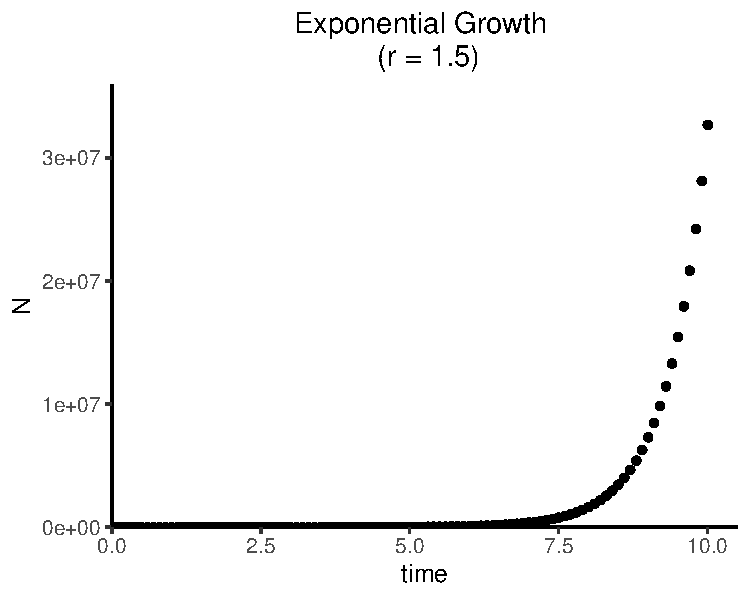
\includegraphics[width=0.7\linewidth]{02_Week_2_files/figure-latex/unnamed-chunk-2-1} \end{center}

\hypertarget{additional-readings-1}{%
\section*{Additional readings}\label{additional-readings-1}}
\addcontentsline{toc}{section}{Additional readings}

\href{./Additional\%20readings/Package\%20deSolve\%20-\%20Solving\%20Initial\%20Value\%20Differential\%20Equations\%20in\%20R.pdf}{Package deSolve: Solving Initial Value Differential Equations in R}

\hypertarget{assignments-1}{%
\section*{Assignments}\label{assignments-1}}
\addcontentsline{toc}{section}{Assignments}

  \bibliography{book.bib,packages.bib}

\end{document}
